% Original-language transcription; see TRANSCRIPTION-NOTES.md.
\documentclass[11pt,a4paper,leqno,twoside]{article}
\usepackage[T1]{fontenc}
\usepackage{lmodern,amsmath,amssymb,tikz}
\usepackage[margin=24mm,headheight=15pt]{geometry}
\usepackage{fancyhdr}
\pagestyle{fancy}\fancyhf{}
\fancyhead[LE,RO]{\thepage}
\fancyhead[CE]{\small HASSLER WHITNEY}
\fancyhead[CO]{\scriptsize FUNCTION NOT CONSTANT ON SET OF CRITICAL POINTS}
\renewcommand{\headrulewidth}{0pt}
\setlength{\parindent}{1.5em}\setlength{\parskip}{3pt}
\setlength{\emergencystretch}{1em}
\newcommand{\sect}[1]{\par\medskip\noindent\textbf{#1}\enspace}
\begin{document}
\setcounter{page}{514}\thispagestyle{plain}
\begin{center}
\textbf{A FUNCTION NOT CONSTANT ON A CONNECTED SET OF\\ CRITICAL POINTS}\par\medskip
By \textsc{Hassler Whitney}
\end{center}
\begingroup\renewcommand{\thefootnote}{}\footnotetext{Received May 16, 1935; presented to the American Mathematical Society, October 26, 1935. The example given here was discovered in 1932 while the author was a National Research Fellow.}\endgroup
\sect{1. Introduction.} Let $f(x_1,\ldots,x_n)$ be a function of class $C^m$ (i.e., with continuous partial derivatives through the $m$th order) in a region $R$. Any point at which all its first partial derivatives vanish is called a \textit{critical point} of $f$. Suppose every point of a connected set $A$ of points in $R$ is a critical point. It is natural to suspect then that $f$ is a constant on $A$. But this need not be so. We construct below an example with $n=2$, $m=1$, $A=\text{an arc}$. The example may be extended to the case $n=n$, $m=n-1$, $A=\text{an arc}$. The arc and the function on the arc are easily defined. The extension of the function through the rest of the plane or space is given by a theorem of the author.\footnote{H. Whitney, \textit{Analytic extensions of differentiable functions defined in closed sets}, Transactions of the American Mathematical Society, vol.\ 36 (1934), pp.\ 63--89, Lemma 2. We refer to this paper as AE.}

The question settled in this paper was raised implicitly in a paper of W. M. Whyburn.\footnote{W. M. Whyburn, Bull. Amer. Math. Soc., vol.\ 35 (1929), pp.\ 701--708.} It is brought up by his definition of critical sets as the maximal connected subsets of the set of critical points on which the function takes a single critical value. Theorem 2 of Whyburn's paper shows that an example of the type given in the present paper can be constructed only by using critical sets which have points that cannot be joined in these sets by rectifiable arcs. It would be interesting to discover how far from rectifiable a closed set must be to be a set of critical points of some function but not a critical set of the function. It may be remarked that any closed set may be a critical set.\footnote{See A. Ostrowski, Bull. des Sciences Math., Feb.\ (1934), pp.\ 64--72.}

For fixed $n$ and $m$ large enough, $m\geq[(n-3)^2/16+n]$, where $[n]$ is the integral part of $n$, $f$ must be constant on any connected critical set, as shown by M. Morse and A. Sard in an unpublished paper.

The example shows that it is in general impossible to express the values of a function $f(x_1,\ldots,x_n)$ along a curve which is not rectifiable by means of an integral of a function of partial derivatives of $f$ of order $\leq n-1$ along the curve.\footnote{For such an expression (using partial derivatives of any desired order) along a rectifiable curve, see H. Whitney, \textit{Functions differentiable on the boundaries of regions}, Annals of Mathematics, vol.\ 35 (1934), pp.\ 482--485, (1) and (3).}

\sect{2. The arc.} Let $Q$ be a square of side 1 in the plane. Let $Q_0$, $Q_1$, $Q_2$, $Q_3$ be squares of side $1/3$ lying interior to $Q$ in cyclical order, each a distance $1/12$

\newpage % Original page 515
\noindent from the boundary of $Q$. Let $q$ and $q'$ be the centers of the sides of $Q$ along $Q_0$, $Q_1$, and along $Q_3$, $Q_0$. Let $q_i$ and $q'_i$ be centers of adjacent sides of $Q_i$ ($i=0,1,2,3$) so that $q'_{i-1}$ and $q_i$ face each other ($i=1,2,3$), and $q_0$ is near $q$, $q'_3$ is near $q'$. Let $A_0$ be a line joining $q$ and $q_0$, let $A_i$ join $q'_{i-1}$ and $q_i$ ($i=1,2,3$), and let $A_4$ join $q'_3$ and $q'$.

Suppose we have constructed squares $Q_{i_1\cdots i_t}$, points $q_{i_1\cdots i_t}$, $q'_{i_1\cdots i_t}$, and lines $A_{j_1\cdots j_t}$ (each $i_k=0,1,2,3$; each $j_k=0,1,2,3,4$) for $t<s$. By taking a square $Q_{i_1\cdots i_{s-2}}$, shrinking it to a third its size, and turning it around and upside down if necessary, we may place it in $Q_{i_1\cdots i_{s-1}}$ so that $q_{i_1\cdots i_{s-2}}$ and $q'_{i_1\cdots i_{s-2}}$ go into $q_{i_1\cdots i_{s-1}}$
\begin{center}
% Vector reconstruction of the original diagram, retaining its labels and incidences.
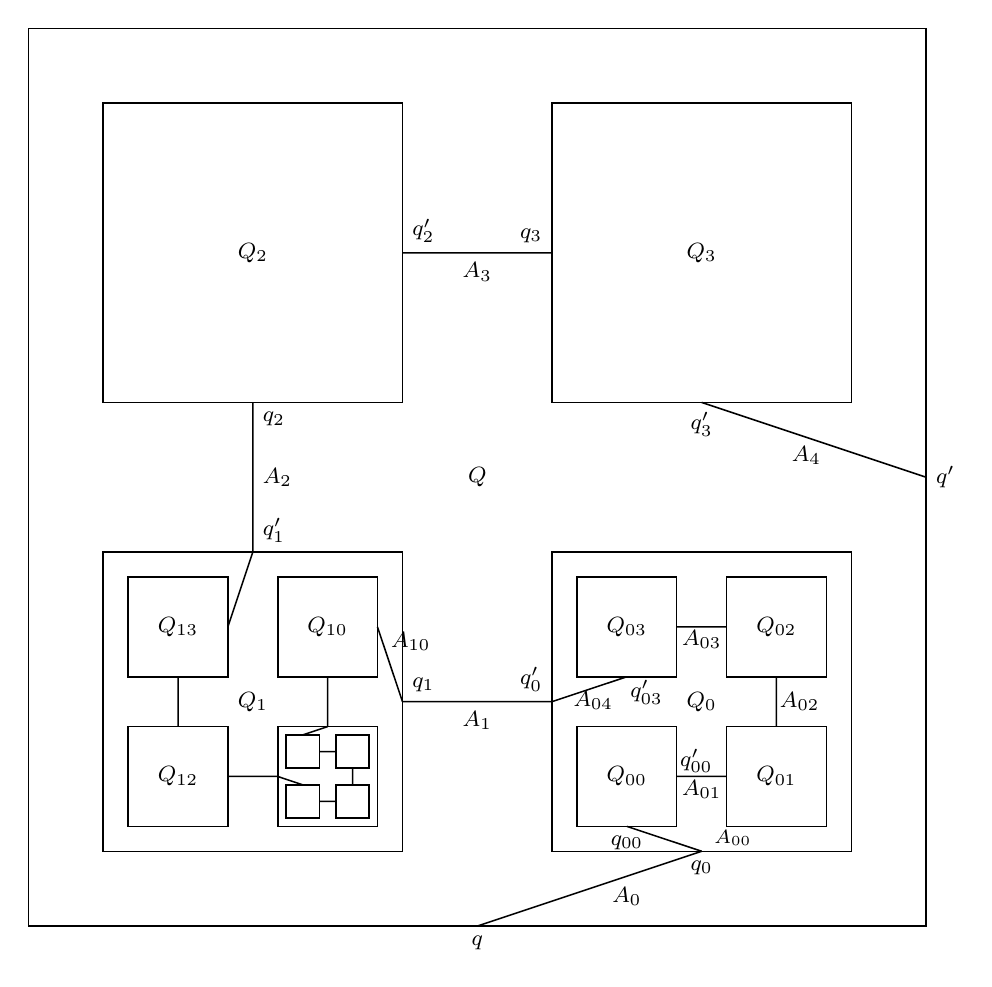
\begin{tikzpicture}[x=.95cm,y=.95cm,line width=.55pt,font=\footnotesize]
\draw (0,0) rectangle (12,12);
\foreach \x/\y/\lab in {7/1/0,1/1/1,1/7/2,7/7/3}{\draw (\x,\y) rectangle +(4,4);}
\draw (6,0)--(9,1) (7,3)--(5,3) (3,5)--(3,7) (5,9)--(7,9) (9,7)--(12,6);
\node at (6,6){$Q$};\node at (3,9){$Q_2$};\node at (9,9){$Q_3$};
\node[below] at (6,0){$q$};\node[right] at (12,6){$q'$};
\node[below] at (9,1){$q_0$};\node[above left] at (7,3){$q'_0$};
\node[above right] at (5,3){$q_1$};\node[above right] at (3,5){$q'_1$};
\node[below right] at (3,7){$q_2$};\node[above right] at (5,9){$q'_2$};
\node[above left] at (7,9){$q_3$};\node[below] at (9,7){$q'_3$};
\node[below] at (8,.65){$A_0$};\node[below] at (6,3){$A_1$};
\node[right] at (3,6){$A_2$};\node[below] at (6,9){$A_3$};\node[below] at (10.4,6.55){$A_4$};
\foreach \x/\y/\lab in {7.333/1.333/00,9.333/1.333/01,9.333/3.333/02,7.333/3.333/03,3.333/3.333/10,1.333/1.333/12,1.333/3.333/13}{
\draw (\x,\y) rectangle +(1.333,1.333);\node at (\x+.666,\y+.666){$Q_{\lab}$};}
\draw (3.333,1.333) rectangle (4.666,2.666);
\draw (9,1)--(8,1.333) (8.666,2)--(9.333,2) (10,2.666)--(10,3.333) (9.333,4)--(8.666,4) (8,3.333)--(7,3);
\node at (9,3){$Q_0$};\node[below] at (8,1.333){$q_{00}$};
\node[above right,inner sep=1pt] at (8.666,2){$q'_{00}$};
\node[below right,inner sep=1pt] at (8,3.333){$q'_{03}$};
\node[anchor=west,inner sep=.3pt,font=\scriptsize] at (9.15,1.18){$A_{00}$};
\node[below,inner sep=1pt] at (9,2){$A_{01}$};
\node[right,inner sep=1pt] at (10,3){$A_{02}$};
\node[below,inner sep=1pt] at (9,4){$A_{03}$};
\node[below,inner sep=1pt] at (7.55,3.18){$A_{04}$};
\draw (5,3)--(4.666,4) (4,3.333)--(4,2.666) (3.333,2)--(2.666,2) (2,2.666)--(2,3.333) (2.666,4)--(3,5);
\node at (3,3){$Q_1$};\node[right,inner sep=1pt] at (4.8,3.8){$A_{10}$};
\foreach \x/\y in {3.444/2.111,4.111/2.111,4.111/1.444,3.444/1.444}{\draw (\x,\y) rectangle +(.444,.444);}
\draw (4,2.666)--(3.666,2.555) (3.888,2.333)--(4.111,2.333) (4.333,2.111)--(4.333,1.888) (4.111,1.666)--(3.888,1.666) (3.666,1.888)--(3.333,2);
\end{tikzpicture}

\end{center}
\noindent and $q'_{i_1\cdots i_{s-1}}$, and thus construct squares $Q_{i_1\cdots i_s}$, etc. We continue this process indefinitely. Let $Q_{i_1i_2\cdots}$ be the point common to $Q$, $Q_{i_1}$, $Q_{i_1i_2}$, $\ldots$ for each $(i_1,i_2,\ldots)$.

The line segments $A_{i_1\cdots i_s}$ together with the points $Q_{i_1i_2\cdots}$ form an arc $A$. It may be represented as the topological image of the segment $(0,1)$ by letting $A_{i_1\cdots i_s}$ correspond to the segment
\[
\left(\frac{2i_1+1}{9}+\cdots+\frac{2i_{s-1}+1}{9^{s-1}}+\frac{2i_s}{9^s},\quad
\frac{2i_1+1}{9}+\cdots+\frac{2i_{s-1}+1}{9^{s-1}}+\frac{2i_s+1}{9^s}\right),
\]
\newpage % Original page 516
\noindent and letting $Q_{i_1i_2\cdots}$ correspond to the number
\[\frac{2i_1+1}{9}+\frac{2i_2+1}{9^2}+\cdots.\]
\sect{3. The function $f(x,y)$.} We first define $f(x,y)$ along the arc $A$ as follows:
\[
\begin{aligned}
\text{on }A_{i_1\cdots i_s},\quad &f=\frac{i_1}{4}+\cdots+\frac{i_s}{4^s};\\[8pt]
\text{at }Q_{i_1i_2\cdots},\quad &f=\frac{i_1}{4}+\frac{i_2}{4^2}+\cdots.
\end{aligned}
\]
$f$ increases from 0 to 1 as we run along $A$ from $q$ to $q'$. Set $f_{00}(x,y)=f(x,y)$, $f_{10}(x,y)=f_{01}(x,y)=0$ on $A$. We shall show that \textit{$f_{00}$ is of class $C^1$ on $A$ in terms of $(f_{00},f_{10},f_{01})$} (see AE). It will follow from Lemma 2 of AE that the definition of $f(x,y)$ may be extended over the plane (in particular, over $Q$) so that $f$ is of class $C^1$; also $\partial f/\partial x=f_{10}=0$, $\partial f/\partial y=f_{01}=0$ on $A$, and hence each point of $A$ is a critical point of $f$.

As $f_{10}$ and $f_{01}$ are continuous in $A$, we need merely prove that for each $\epsilon>0$ there is a $\delta>0$ such that if $(x,y)$ and $(x',y')$ are points of $A$ whose distance apart is $r<\delta$, then
\begin{equation}\tag{1}|f(x',y')-f(x,y)|<r\epsilon,\end{equation}
(see AE (3.1) and (3.2)).

The proof rests on the following two facts.

(a) If $(x,y)$ and $(x',y')$ are points of $A\cap Q_{i_1\cdots i_s}$, then
\begin{equation}\tag{2}|f(x',y')-f(x,y)|\leq1/4^s.\end{equation}
(b) If $(x,y)$ and $(x',y')$ are points of $A$ separated by some point $Q_{i_1i_2\cdots}$, and if $Q_{i_1\cdots i_s}$ is the smallest square containing them both, then
\begin{equation}\tag{3}r>\frac1{12}\frac1{3^{s+1}}.\end{equation}
Assume (a) and (b) are true. Given $\epsilon>0$, choose $s_0$ and $\delta$ so that
\begin{equation}\tag{4}36\left(\frac34\right)^{s_0}<\epsilon,\qquad\delta<\frac1{12}\frac1{3^{s_0+1}}.\end{equation}
Now let $(x,y)$ and $(x',y')$ be any two points of $A$ distant $r<\delta$. If no point $Q_{i_1i_2\cdots}$ separates them, then $f(x',y')=f(x,y)$, and (1) holds. Otherwise, let $Q_{i_1\cdots i_s}$ be the smallest square containing them both. (b) gives
\[\frac1{12}\frac1{3^{s+1}}<r<\delta<\frac1{12}\frac1{3^{s_0+1}},\quad\therefore s>s_0.\]
Hence
\[\frac{|f(x',y')-f(x,y)|}{r}\leq\frac{12\cdot3^{s+1}}{4^s}=36\left(\frac34\right)^s<\epsilon.\]
\newpage % Original page 517
It remains to prove (a) and (b). (a) is obvious from the definition of $f$. To prove (b), we consider three cases: neither point is in any square $Q_{i_1\cdots i_s i_{s+1}}$; each point is in such a square; one point is in such a square, and the other is not. In the first two cases we see that $r>1/(2\cdot3^{s+1})$; in the third case, (3) holds.

\sect{4. Generalization to higher dimensions.} We shall indicate how the corresponding example is constructed for $n=3$, $m=2$; the generalization to higher dimensions is obvious.

Let $Q$ be a cube of side 1. Let $Q_0,\ldots,Q_7$ be cubes of side $2/5$ arranged in $Q$ so that $Q_i$ is adjacent to $Q_{i-1}$. Let $q$ and $q'$ be the centers of faces of $Q$ which are adjacent and adjacent respectively to $Q_0$ and $Q_7$. Define $q_i$ and $q'_i$ ($i=0,\ldots,7$) as before, and similarly for $A_0,\ldots,A_8$. The process is continued indefinitely, as before. $A$ is again an arc. We set
\[
\begin{aligned}
\text{on }A_{i_1\cdots i_s},\quad &f=\frac{i_1}{8}+\cdots+\frac{i_s}{8^s},\\[8pt]
\text{at }Q_{i_1i_2\cdots},\quad &f=\frac{i_1}{8}+\frac{i_2}{8^2}+\cdots.
\end{aligned}
\]
Set $f_{000}=f$, $f_{\alpha\beta\gamma}=0$ ($\alpha+\beta+\gamma=1$ or 2) on $A$. To prove that $f=f_{000}$ is of class $C^2$ in terms of these functions we need merely show that
\begin{equation}\tag{5}\Delta=|f(x',y',z')-f(x,y,z)|<r^2\epsilon\text{ on }A\qquad(r<\delta).\end{equation}
Note that $f$ varies by at most $1/8^s$ in any $Q_{i_1\cdots i_s}$. Now if the smallest cube containing $(x,y,z)$ and $(x',y',z')$ is $Q_{i_1\cdots i_s}$, $r$ is of the order $(2/5)^s$, while $\Delta\leq1/8^s$; hence $\Delta/r^2$ is of the order $(25/32)^s$, which is $<\epsilon$ for $r$ small enough and hence $s$ large enough.

Note that \textit{all partial derivatives of $f$} (of order $\leq n-1=2$) \textit{vanish on $A$}.

\medskip\textsc{Harvard University.}
\end{document}
